% -*- root: ../main.tex -*-

% Esporre i principali problemi affrontati durante l'effettiva realizzazione delle componenti hardware/software e illustrare le soluzioni implementative adottate. Se l'elaborato ha previsto l'utilizzo di tecnologie già disponibili sul mercato, discuterne brevemente le caratteristiche e motivarne l'adozione rispetto ad altre soluzioni assimilabili. NOTA: in questa sezione devono essere riportate esclusivamente le porzioni di codice ritenute particolarmente significative.
% 10000 - 21000 battute

\chapter{Implementazione}
\section{Software Microcontrollori}
\paragraph{Classe principale}
Come spiegato nel capitolo Scelte tecnologiche cruciali, i microcontrollori sono stati programmati in \textbf{MicroPython}. Nella classe principale, condivisa e riutilizzabile tra tutti i microcontrollori, dopo la connessione a internet e al broker MQTT è stato creato uno \textbf{scheduler}.  Questo si occupa di eseguire i \textbf{task a lui assegnati}, siano relativi al cibo, all'acqua, o ai parametri vitali. 
In questo modo è facilmente programmabile il comportamento di un microcontrollore con task modulari.
    \begin{lstlisting}
        # array of tasks
        print("Creating array of tasks")
        tasks = [smart_collar_temperature_task.get_behaviour(), smart_collar_heartbeat_task.get_behaviour()]  # array of coroutines
        
        # create the scheduler and start tasks
        print("--- Starting Scheduler ---")
        scheduler = Scheduler()
        scheduler.start(tasks)
    \end{lstlisting}
    

    \paragraph{Classi per sensori e attuatori}
    Avendo adottato MicroPython è stato possibile usufruire del linguaggio ad oggetti per modellare attuatori e sensori come classi, con proprietà chiamabili all'occorrenza. Ogni classe è stata testata individualmente grazie ai test scritti appositamente per prevenire comportamenti indesiderati. Si può trovare il diagramma delle classi di ogni device con cui si interfaccia il microcontrollore in [Fig. \ref{fig:classdiagram}]. 
    
    \begin{figure}[H]
        \caption{Diagramma delle classi}
        \label{fig:classdiagram}
        \centering
        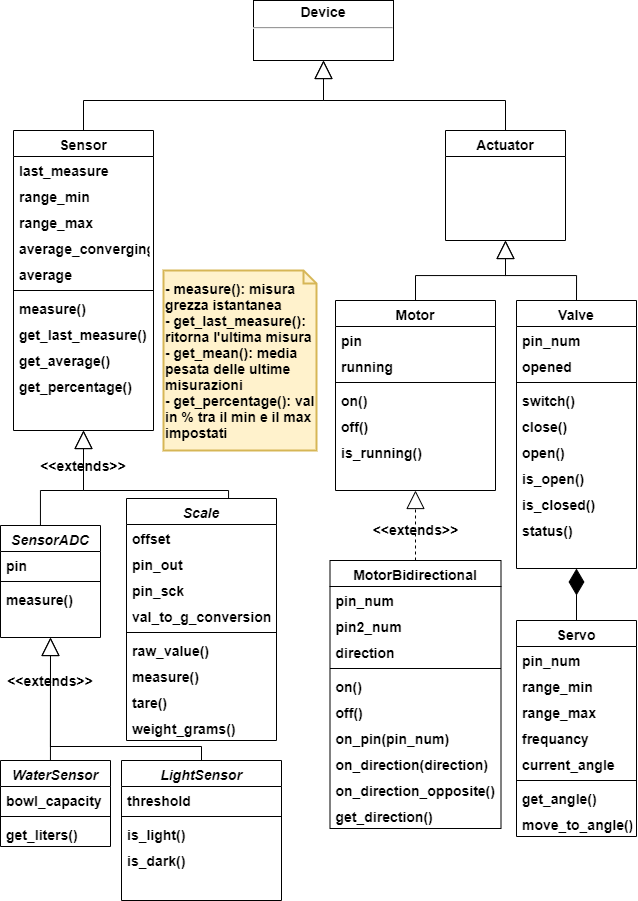
\includegraphics[width=0.8\textwidth]{DrawIo/ClassDiagram.png}
    \end{figure}
    
    In particolare, ogni device di sensing, è stato modellato ereditando dalla classe Sensor, che mette a disposizione una serie di metodi per poter calcolare la media pesata, la percentuale misurata nel range minimo e massimo e l'ultima misurazione. La media è pesata è calcolata esponenzialmente in base alle ultime misure, le quali hanno peso maggiore:
    \begin{lstlisting}
    def measure(self):
        """measures 3 times, measure is the mean of them, updates global average, returns measure."""
        sum_raw_measures = 0
        for _ in range(3):
            sum_raw_measures += self.raw_measure()
        self.last_measure = sum_raw_measures / 3
        # average calculated from last average, weighted and actual measure, weighted
        self.average = self.last_measure * self.average_converging_speed +                           self.average * ( 1 - self.average_converging_speed)
        return self.last_measure
    \end{lstlisting}
  
\subsection{Gestione Cibo e Acqua}
    \subsubsection{Cibo}
    L'implementazione del task relativo alla gestione del cibo da passare allo scheduler è stato implementato in una classe dedicata. Il comportamento che il task espone rispecchia la macchina a stati discussa nel design [Fig. \ref{fig:statediagramFood}]. Grazie alla possibilità di Python di avere funzioni higher-order, il loop principale esegue ciclicamente lo stato corrente:
    
    \begin{lstlisting}
        async def get_behaviour(self):
        """ async method called returns a coroutine"""
        while True:
            # executes the current state
            await self.state()
    \end{lstlisting}
    Quando il task è creato, nel costruttore è possibile scegliere lo stato iniziale assegnando la funzione relativa allo stato corrente. 
    \begin{lstlisting}
        # state variable holds the current state, this is the initial state
        self.state = self.check_food_consumption
    \end{lstlisting}
    All'interno di ogni stato vengono effettuate le operazioni necessarie e, qualora le condizioni si verifichino, le transizioni a un nuovo stato.
    \begin{lstlisting} 
        # check consumption
        self.reduction_percentage = self.previous_sent_perc - self.scale.get_percentage()
        print("\t\tReduction Percentage: {:.2f}".format(self.reduction_percentage))
        if self.reduction_percentage >= PERCENTAGE_CONSUMPTION_THRESHOLD:
            self.state = self.send_food_consumption
            return
    \end{lstlisting}
    Particolarmente impegnativa è stata la modellazione della bilancia. Questa va tarata inizialmente affinché il peso della ciotola vuota non vada ad influire sul peso del cibo. Inoltre parecchie prove sono state effettuate per trovare il coefficiente di conversione tra i valori del sensore e il peso in grammi.
    Infine la gestione del motore bidirezionale per aprire e chiudere lo sportellino di accesso al cibo ha anch'esso richiesto parecchia cura, dovendo implementare una classe che si preoccupasse di invertire la polarità al motore attraverso un ponte-H e la logica di interruzione del movimento al momento giusto. 
    
    \subsubsection{Acqua}
    Il task relativo alla gestione della ciotola dell'acqua è stato implementato, similmente a quello del cibo, in una classe apposita, per poter essere passato allo scheduler. Essendo i task più di uno, a questo punto è sorto naturale implementare una classe task da cui tutti quelli descritti nel seguente capitolo erediteranno.
    La logica a stati del design è stata implementata rispecchiandolo a pieno. Ciò perché la precedente modellazione dei sensori ha agevolato di parecchio la scrittura del codice, rendendolo pulito e facilmente comprensibile. 
    \begin{lstlisting} 
        # measure
        self.waterSensor.measure()
        print("\t\t\tWater Measure:  {:.2f}".format(self.waterSensor.get_percentage()))
        # check empty
        if self.waterSensor.get_percentage() < self.min_water_lvl_perc:
            print("\t\t\tWater LOW: {:.2f} < {:.2f}".format(self.waterSensor.get_percentage(), self.min_water_lvl_perc))
            if self.valve_present:
                print("\t\t\tOpening Valve")
                self.valve.open()
                self.state = self.fill_water_bowl
                return
    \end{lstlisting}
    In questo caso il sensore dell'acqua è stato ampliato con delle funzioni per il ritorno della percentuale. Non è possibile infatti dedurre il quantitativo bevuto da un'animale semplicemente dal sensore, poiché il range di questo è proporzionale all'altezza del liquido nel contenitore, ma non è dato sapere la sua capienza. Per questo motivo il parametro capienza massima può essere passato al dispositivo di sensing. Grazie a questo dato verrà calcolata la quantità di acqua bevuta al diminuire della percentuale rilevata dal sensore.
    
    \paragraph{Comunicazioni}
    Entrambi i task di cibo e acqua adottano il protocollo MQTT per comunicare con il cloud. Lo scambio è bidirezionale ed è gestito dalla classe "MQTTManager". Questa si occupa dell'invio dei messaggi e, qualora il task "MQTTMessageChecker" sia in esecuzione, di ricevere i messaggi dal server. Questi messaggi innescheranno la gestione delle callback passando allo scheduler un task "MQTTMessageHandler".
    I messaggi sono scambiati in formato JSON. 
    Ogni unità di controllo gabbia inizialmente si identifica mandando un messaggio al broker. In seguito vengono iniziate le rilevazioni per i consumi e, in caso di necessità, un messaggio affinché il server invii la notifica all'addetto.
    \begin{figure}[H]
        \caption{Sequenza scambio dei messaggi del sistema acqua}
        \label{fig:sequencewater}
        \centering
        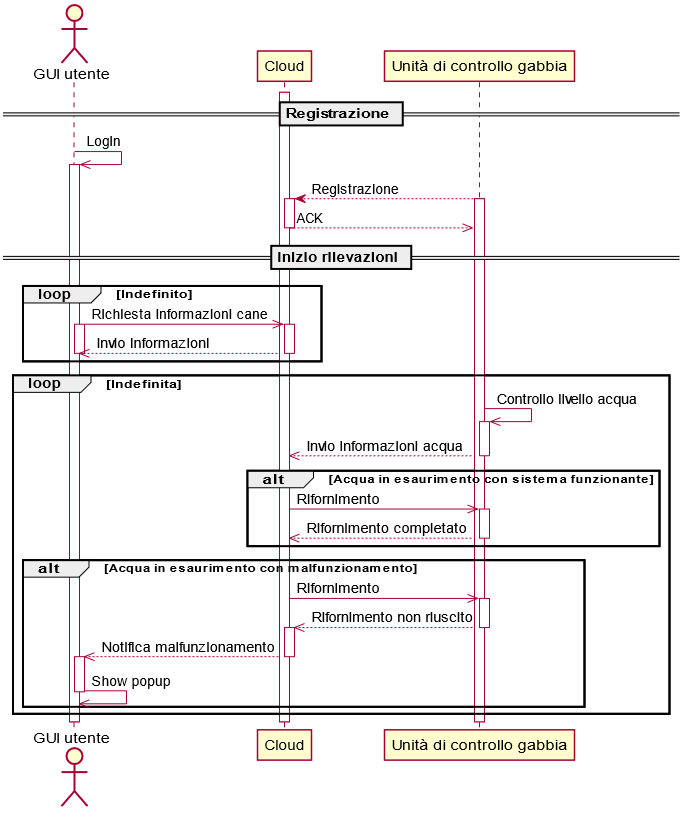
\includegraphics[width=0.8\textwidth]{DrawIo/sequenceWaterAutomation.png}
    \end{figure}

\subsection{Monitoraggio Parametri Vitali}
\subsubsection{Temperatura}
Il task relativo al monitoraggio della temperatura nel collare è stato sviluppato affinché possa essere usato con due sensori diversi: il ds18x20 e il dht11. 
Creando il task si può scegliere il modello posseduto e, quando lo scheduler inizierà a eseguire ciclicamente le misurazioni, i dati e le notifiche verranno inviati in cloud.
    \begin{lstlisting} 
        # measure temp
        if self.using_ds18x20:
            temp = self.check_ds18x20()
        else:
            temp = self.check_dht()
        # send data
        self.mqtt_manager.send_msg(self.topic, "Temperature: {}".format(temp))
    \end{lstlisting}

\subsubsection{Battito Cardiaco}
Il task relativo al battito cardiaco svolge, come il precedente, delle misurazioni cicliche e invia i dati rilevati.
Un parte particolarmente complessa è stata quella della gestione del sensore per il battito. Il sensore, qualora interpellato, fornisce un singolo valore direttamente proporzionale alla dilatazione dei vasi sanguigni. Ne deriva la necessità di attuare misurazioni frequenti per non incorrere nella perdita della breve variazione di un battito. Abbiamo stabilito la frequenza di campionamento in base a quanto segue:
Considerando che in condizioni di riposo, i battiti per minuto di un cane - da intendersi come pulsazioni - sono generalmente compresi tra 60 e 140 bpm, in base alla taglia, età e razza, e il valore può raggiungere valori anche più alti qualora in movimento, abbiamo preso come valore limite da rilevare 150 bpm. Ciò, significa che il tempo di ogni ciclo cardiaco $T_{cc}$ è:
\begin{equation}
T_{cc} = \frac{1}{bps} = \frac{1}{\frac{bpm}{60}}= \frac{60}{bpm} \Rightarrow \frac{60}{150 bpm} = 0.4s
\end{equation}
Considerato che il ciclo cardiaco si compone in sistole (contrazione) e diastole (rilassamento), la fase sistolica è quella più facilmente rilevabile poiché la contrazione ventricolare causata è più violenta e breve. Questa fase durante le rilevazioni effettuate dura circa un mezzo del ciclo cardiaco e produce un picco nei valori particolarmente indicativo per rilevare il battito in mezzo al naturale rumore del sensore. Per non perdere il picco massimo il numero di campionamenti $N_{c}$ durante questa fase è stato fissato a 20. La frequenza di campionamento minima risultante $f_{min}$ è stata calcolata come: 
\begin{equation}
f_{min} = \frac{ \frac{1}{2} *  T_{cc} }{N_{c}} \Rightarrow  \frac{ \frac{1}{2} *  0.4s }{20} = 0.01s = 10 ms 
\end{equation}

Salvando i valori risultanti e graficandoli con la libreria python "Mathplotlib" si ottiene una linea come quella di colore rosso in [Fig. \ref{fig:Heartbeat}]. Si può notare che il campionamento è sufficiente e permette di distinguere intuitivamente i battiti. 
Per rilevare le pulsazioni a livello digitale però è necessario formalizzare un altro modello matematico che non faccia incorrere il sistema in falsi positivi o falsi negativi. Un primo approccio si è basato su stabilire una singola soglia, oltre la quale il battito è rilevato e registrato. Questa soluzione si è rivelata inadatta in quanto il disturbo del sensore la farebbe attraversare più volte (si veda in [Fig. \ref{fig:Heartbeat}] poco prima del campionamento numero 2400 il valore attraversa la linea azzurra parecchie volte). Inadatti si sono rivelati anche i tentativi di normalizzare la linea dei valori, in quanto parecchio discontinui e di frequenza elevata, si perde la differenziazione dei picchi. Si è optato per stabilire una doppia soglia, la prima, più alta, oltre la quale il battito è rilevato, la seconda, più bassa, che determina la fine del battito. La prima volta che il valore attraversa la prima [Fig. \ref{fig:Heartbeat}, linea azzurra] una variabile registra il battito e nessun altra registrazione viene effettuata sino a che i valori non scendono sotto la soglia di fine battito [Fig. \ref{fig:Heartbeat}, linea gialla]. 
Queste soglie non possono essere fisse, variando la pressione di animale in animale e pure di giorno in giorno per lo stesso essere vivente. Per questo motivo i valori sono stati fissati per la prima a 4/5 e per la seconda a 1/2 tra minimo [Fig. \ref{fig:Heartbeat}, linea verde] e massimo [Fig. \ref{fig:Heartbeat}, linea blu] dei precedenti valori. La grandezza della finestra dei valori da cui prendere minimo  e massimo è stata fissata a 250 valori. Questo perché, come si può notare dal grafico, comprende almeno due battiti. Un range troppo piccolo creerebbe dei minimi e massimi locali, rilevando picchi non propri e dando parecchi falsi positivi. Una finestra troppo ampia porterebbe a una staticità delle soglie rispetto alla variazione di pressione che creerebbe falsi negativi.  

    %GRAFICO BATTITO
    \begin{figure}[H]
        \caption{Grafico Battiti}
        \label{fig:Heartbeat}
        \centering
        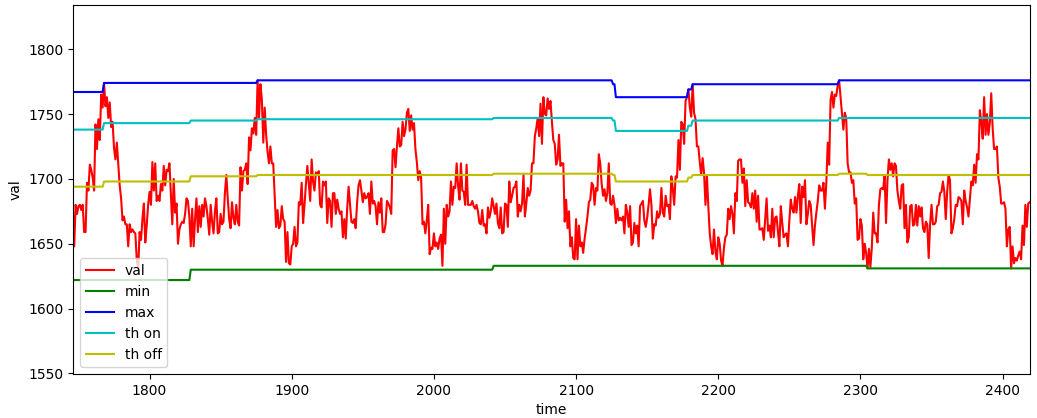
\includegraphics[width=1\textwidth]{Images/heartbeatGraph.png}
    \end{figure}
    \begin{lstlisting}
       val = self.pulse_sensor.raw_measure()
        self.history.append(val)  # add to history of values
        # crop to MAX_HISTORY length, getting the tail (last ones)
        self.history = self.history[-MAX_HISTORY:]
        # get min max in the history
        minima, maxima = min(self.history), max(self.history)
        # get thresholds
        threshold_on = (minima + maxima * 4) // 5  # 4/5
        threshold_off = (minima + maxima) // 2  # 1/2
        # if val goes above beat threshold and no beat has previously been detected.
        if val > threshold_on and self.still_beat == False:
            # beat detected
            self.led.on()
            self.still_beat = True  # prevents multiple appends for all the measures during a beat
            # once every beat
            self.beats.append(time.time())
    \end{lstlisting}

Una volta rilevati i singoli battiti con il modello matematico, il calcolo del battiti al minuto è stato realizzato salvando la cronologia degli istanti di tempo per gli ultimi N battiti $N_{beats}$. Sperimentalmente si è optato per 30 registrazioni per mantenere il valore dei bpm reattivo ma non dipendente solo da poche unità. Prelevando dalla cronologia il tempo passato $T_{diff}$ per questi battiti, si può facilmente derivare il rateo di $bpm$ attuale tramite la formula: 
\begin{equation}
bpm = \frac{ N_{beats}*60 s/min }{T_{diff}} = \frac{ N_{beats}*60 s/min }{T_{last}-T_{first}} 
\end{equation}
Il battito cardiaco risultante viene poi inviato periodicamente al Database e, qualora ci fossero anomalie, una notifica viene invece generata e inviata immediatamente.
    \begin{lstlisting}
        # calculate bpm
        beats_time = self.beats[-1] - self.beats[0]  # time difference between end and start of the queue
        if beats_time:
            bpm = (len(self.beats) / beats_time) * 60
            print("HeartBeat: {}".format(bpm))
            # if outside range
            if bpm < self.min_heartbeat or bpm > self.max_heartbeat:
                # send notification now
                self.mqtt_manager.send_msg(MQTT_NOTIFY_TOPIC, ujson.dumps({"Notify":"Heartbeat is abnormal: {}".format(bpm)}))
    \end{lstlisting}

\paragraph{Comunicazioni}
    I task di temperatura e battiti adottano anch'essi il protocollo MQTT per comunicare con il cloud. Lo scambio è bidirezionale per via della necessità di settare i range di temperatura e battiti per le notifiche di anomalia.
    Ogni unità collare inizialmente si identifica mandando un messaggio al broker. Successivamente partono le rilevazioni per i battiti e la temperatura. I parametri vitali vengono periodicamente inviati al server assieme ai messaggi per le notifiche di anomalie.
    \begin{figure}[H]
        \caption{Sequenza scambio dei messaggi del sistema collare}
        \label{fig:sequencesmartcollar}
        \centering
        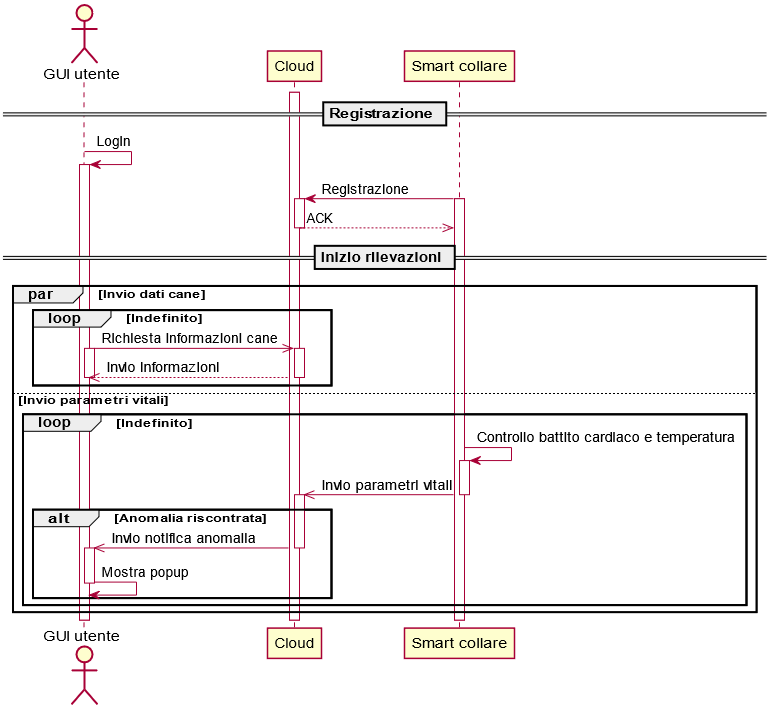
\includegraphics[width=0.8\textwidth]{DrawIo/sequenceSmartCollar.png}
    \end{figure}
    
\section{Software Videosorveglianza}
Il Raspberry è stato scelto come board per la computazione delle immagini di video-sorveglianza. Il principale concorrente a questa scelta, l'ESP32-CAM è stato testato per lo streaming video ma non è provvisto delle risorse computazionali necessarie per il rilevamento di anomalie. 
Ciononostante, avendo un costo inferiore rispetto al Raspberry è stato comunque considerato come alternativa low-cost. 
Il linguaggio scelto per la programmazione è stato \textbf{Python} per continuità con i microcontrollori e per la flessibilità di utilizzo. 
Sono state programmate multiple classi per di complessità crescente per agevolare l'utilizzo del software in caso di errori.
La prima classe "camera tester" ha infatti semplicemente il ruolo di testare lo stream con ffmpeg e OpenCV.
Un'altra classe "mqtt tester" si occupa di un semplice test di invio e ricezione attraverso il pacchetto mqtt di "awsiotsdk". 
Infine l'ultima classe di test "stream base" si occupa di testare lo stream attraverso l'utilizzo del pacchetto "flask" per creare un webserver su cui verrà pubblicato il video feed.
\paragraph{Comunicazione}
La parte di comunicazione è stata gestita creando una classe MQTT apposita che permette di connettersi, disconnettersi, mandare dei messaggi e impostare le callback. Questa classe viene usata da tutte le classi successive per le comunicazioni.
Infine, per passare lo stream video da un dispositivo ad un altro nella stessa rete, sono state incluse due classe "sender udp" e "receiver udp" atte allo scopo.

\subsection{Motion Detection}
Una delle due implementazioni proposte per il rilevamento di anomalie utilizza la motion detection. Questa tecnica si basa sul rilevare i cambiamenti dell'immagine corrente dato uno sfondo di riferimento.
Il motion detector base è stato costruito come segue:
Viene preso il frame corrente e viene sfumato con un filtro gaussiano per rimuovere minime differenze.
Il risultato viene sottratto al frame di riferimento per il background. 
Nel nostro caso il frame di riferimento per il background viene aggiornato periodicamente. 
L'immagine che contiene le differenze viene passata attraverso una soglia per rilevare le zone con cambiamenti sostanziali e non minimi.
Viene applicata la dilatazione per unire le zone discontinue in modo tale da unire aree vicine di cambiamento. 
Viene calcolata l'area delle zone di differenza e vengono scelte solo le zone con un'area maggiore di una soglia. 
Le zone scelte sono zone effettive di cambiamento dell'immagine. 
    \begin{lstlisting}
    # blur
    gray_frame = cv2.GaussianBlur(gray_frame, (21, 21), 0)
    # compute the absolute difference between the current frame and reference frame
    frameDelta = cv2.absdiff(referenceFrame, gray_frame)
    thresh = cv2.threshold(frameDelta, 25, 255, cv2.THRESH_BINARY)[1]
    # dilate the thresholded image to fill in holes, then find contours
    # on thresholded image
    thresh = cv2.dilate(thresh, None, iterations=2)
    cnts = cv2.findContours(thresh.copy(), cv2.RETR_EXTERNAL,
                            cv2.CHAIN_APPROX_SIMPLE)
    \end{lstlisting}
Il motion detector base è stato ampliato in altre due classi per comprendere l'invio di messaggi MQTT al rilevamento di un movimento ("motion detection mqtt") e lo streaming video assieme all'invio di messaggi ("motion detection mqtt stream"). 

\subsection{Object Detection}
La seconda implementazione proposta per la rilevazione di anomalie o intrusioni nel sistema di videosorveglianza fa uso di reti neurali per l'object detecion. 
La classe "object detection base" fa uso della rete neurale Yolo (una più approfondita discussione sulla scelta delle reti è presente nel capitolo Testing) per predire la presenza di oggetti anomali nella scena.
Il codice permette di venir usato per il forward alla rete di una singola immagine, di un video, o di uno streaming da webcam. Nel mentre vengono calcolati i tempi di computazione per derivare gli FPS a cui il sistema sta andando.
Assieme a questa classe è stata implementata la variante "object detection mqtt" con l'invio su MQTT del messaggio di anomalia e dell'oggetto rilevato per la notifica.

    \begin{lstlisting}
            # capture frame
            ret, image = cap.read()

            #predition
            boxes, confidences, classIDs, idxs = make_prediction(net, layer_names, labels, image, args.confidence, args.threshold)
            #draw boxes
            image = draw_bounding_boxes(image, boxes, confidences, classIDs, idxs, colors)
    \end{lstlisting}


\section{Web App}

    La \textbf{Web App} è stata sviluppata come un prototipo funzionante, ma che per essere considerato completo richiederebbe ancora lavoro di rifinitura.
    
    \subsection{Considerazioni tecnologiche}
    
        L'applicazione è stata sviluppata utilizzando \textbf{nodeJS} e \textbf{VueJS}. 
        Una scelta guidata dalla semplicità del framework javascript, che a differenza di \textbf{React} e \textbf{Angular} offre una curva di apprendimento ben più bassa, favorendo lo sviluppo. 
        \textbf{VueJS} forniva inoltre il vantaggio di integrarsi perfettamente con AWS \textbf{Amplify}, a livello di \textbf{front-end}.
        Mentre a livello di \textbf{back-end} le comunicazioni sono perfettamente supportate dato che anche l'applicativo \textbf{back-end} è stato sviluppato con \textbf{nodeJS}.
        
        Il comparto estetico è sviluppato utilizzando \textbf{Vuetify}, questa è un'estensione di \textbf{VueJS} che sembrava integrarsi meglio con il framework rispetto a \textbf{BootstrapVue}.
        
        Per la comunicazione con le API \textbf{REST} si è scelto di utilizzare \textbf{AXIOS} rispetto ad \textbf{AJAX}, questo perché risulta di facile integrazione con \textbf{VueJS}, supporta le \textbf{SPA} e consente il facile utilizzo di \texttt{Async} e \texttt{Await}.
        
        Mentre per le \texttt{websocket} si è scelto di usare le librerie di default, principalmente per la loro semplicità di utilizzo. È stata valutata l'adozione di \texttt{Socket.io} che forniva maggiori funzionalità  e supporto a comunicazioni come l'utilizzo di \texttt{fall back}.
        Tali funzionalità, tuttavia, non erano utili per un utilizzo così basilare, pertanto l'idea di utilizzare questa libreria è stata accantonata.
        
        Per quanto riguarda le \texttt{route} della pagina è stato utilizzato \textbf{VueRouter}, essendo l'unica alternativa.
        
        Infine per facilitare lo sviluppo è stato utilizzato \textbf{Vuex} che consente di accedere da più punti ad un oggetto condiviso.
        
    \subsection{Note sul codice}
        Per questioni di velocità e leggibilità si è deciso di dividere l'applicativo su più \texttt{view} : \textbf{Home} e \textbf{Login}.
        
        Ogni \texttt{view} è composta da più componenti che a loro volta sono composti.
        
        Tutti gli elementi di \textbf{VueJS} sono stati strutturati seguendo il modello del \textbf{Single File Components} che prevede di inserire il codice per lo \textbf{Style}(CSS), \textbf{Markup}(Vue/HTML) e \textbf{Script}(JavaScript) tutto nello stesso file.
        
    \subsection{Difficoltà durante lo sviluppo}
    
        Lo sviluppo della \textbf{Web App}  è stato fluido fino all'integrazione della prima chiamata alle \textbf{API}. Qui ci si è resi conto che le api non potevano essere chiamate direttamente dal \textbf{Browser}, mentre funzionavano perfettamente utilizzando sistemi come \textbf{Postman} e \textbf{Reqbin}. 
        
        E' stato più volte riscontrato l'errore \textbf{Cross-Origin Resource Sharing} (CORS), che riguarda la possibilità di utilizzare altre sorgenti per attingere alle informazioni. Questo genere di verifica viene effettuata solo dal Browser ed è invece saltata su Postman e simili.
        
        Dopo un investigazione siamo giunti alla conclusione che in fase di \textbf{sviluppo} avremmo potuto consentire ogni richiesta. Abbiamo quindi aggiunto le seguenti linee di codice nel file \texttt{Template.yaml} di \textbf{SAM},  per istruire il proxy cors di AWS a rispondere alle richieste con i campi aggiunti:
        \begin{lstlisting}
        Globals:
          Api:
            EndpointConfiguration: REGIONAL
            Cors:
              AllowMethods: "'*'"
              AllowHeaders: "'*'"
              AllowOrigin: "'*'"
        \end{lstlisting}
        
        L'errore ha smesso di presentarsi, ma poiché avevamo la necessità di testare sempre più funzioni e non era pensabile effettuare il deploy di sam per ogni prova, abbiamo iniziato ad eseguire un' istanza di AWS \textbf{Lambda} localmente tramite il comando : \texttt{sam build \&\& sam local start-api}.
        
        Giunti a questo punto il problema si è ripresentato e questa volta la soluzione è stata molto più ostica da trovare, nonostante il problema fosse lo stesso, ovvero la mancanza della risposta \textbf{CORS}.

        %CORS LATO BROWSER
        \begin{figure}[H]
            \caption{Errore lato Broswer}
            \label{fig:ErrorCorsBroswer}
            \centering
            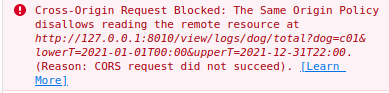
\includegraphics[width=1\textwidth]{Images/CorsErrorFrontEnd.PNG}
        \end{figure}
        
        %CORS LATO CONSOLE
        \begin{figure}[H]
            \caption{Errore lato console}
            \label{fig:ErrorCorsConsole}
            \centering
            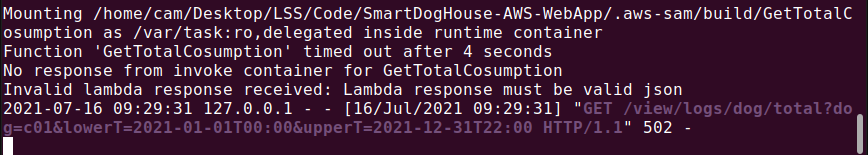
\includegraphics[width=1\textwidth]{Images/CorsErrorConsole.PNG}
        \end{figure}
    
        Volenterosi di utilizzare e testare le funzioni lambda localmente abbiamo cercato una soluzione che risolvesse il problema in maniera esaustiva,
        giungendo finalmente una \href{https://github.com/aws/aws-sam-cli/issues/323#issuecomment-483650280}{Issue} che ha fornito la soluzione se pur non ottimale.
        
        Il comando utilizzato: \texttt{npx lcp --proxyUrl http://localhost:3000/}
        
        La soluzione adottata implica  l'avviare un server proxy CORS che risponda alle richieste \textbf{OPTIONS} e poi reindirizzi all'immagine docker di lambda. 
        Ovviamente la WebApp dovra contattare il proxy e non direttamente il container.
        
        Nonostante gli sviluppatori di SAM confermino il supporto alle chiamate CORS locali non siamo riusciti a farle funzionare in altra maniera.
        
\subsection{Deployment} 
        Il repository è stato collegato e configurato per il continuous deployment, così da pubblicare le modifiche online non appena rilasciate, se il sito compila. Il sito, essendo pubblico, è stato protetto da password con l'utilizzo di Amplify.
        
        
\section{Funzioni Serverless}
    In questa sezione del progetto sono, le principali difficoltà   affrontate sono state legate all'apprendimento delle tecnologie \textbf{AWS} utilizzate:
    \begin{itemize}
        \item \textbf{Lambda}: I due principali problemi incontrati sono stati:
         \begin{itemize}
             \item Lo sviluppo e il testing in locale che richiede l'ausilio della \textbf{SAM CLI} e della \textbf{AWS CLI}.
             \item L'utilizzo del sdk di AWS per javascript, sopratutto quando era necessario contattare altri servizi come IoT Core o API Gateways.
         \end{itemize}
        \item \textbf{IoT Core}: Non sono state riscontrate particolari difficoltà se non con i certificati che non sono in un formato compatibile con la libreria \texttt{UMQTT} di Micropython.
        \item \textbf{CloudWatch}: Consultare i log delle funzioni lambda non risulta complicato, stesso non si può dire per i log delle websocket.
        \item \textbf{IAM}: Il sistema dei permessi di AWS è molto articolato e ci sono più modi per fornire i permessi, in generale la gestione dei permessi è stata faticosa. Alcuni permessi sono molto immediati, altri come quello per consultare i log di \textbf{CloudWatch} delle websocket molto meno, non tanto per i permessi più per il tool grafico o la sintassi di SAM.
        \item \textbf{API gateway}: L'esposizione delle \texttt{API} \textbf{REST} e delle web socket non è stata difficoltosa.
        \item \textbf{SAM}: Forse la parte più complicata dell'applicativo serverless, fornisce la possibilità di effettuare il deploy di \textbf{Stack} su \textbf{AWS CloudFormation}, con una sintassi tutta sua, orchestrare il deploy di : Funzioni Lambda, Regole IoT Core, Permessi IAM, Tabelle DynamoDB, API REST, Websocket e CloudWatch Event via Crono. Nonostante il grande sforzo per sfruttare al meglio SAM, il lavoro potrebbe essere ulteriormente automatizzato e perfezionato. 
    \end{itemize}
    
\subsection{Deployment} 
        L'intero stack che esclude il database principale, Aws Aplify e i dispositivi IOT può essere dispiegato tramite il comando \texttt{sam build \&\& sam deploy}
        Attualmente il deploy è dipendente da alcune variabili che sono configurabili con il flag \texttt{-g}, altre variabili sono incorporate e potrebbero essere scorporate alla stessa maniera se si volesse rendere il deploy multi-account.
        
\section{Database DynamoDB}
        Lo sviluppo del database è una parte critica del progetto,
        in un ottica di rendere l'applicativo veloce e scalabile il più possibile, abbiamo scelto di procedere con lo sviluppo di una tabella DynamoDB.
        DynamoDB offre una scalabilità e una velocità di interrogazione superiori ai database relazionali, per questo lo abbiamo scelto, inoltre la sua prefetta integrazione con il \textbf{back-end} lo rendeva ancora più appetibile.
        
        Le difficoltà durante lo sviluppo del database sono state enormi.
        Partendo dalla documentazione e dalle guide che siamo riusciti a reperire, subito ci siamo trovati in difficoltà con il mindset necessario allo sviluppo del database, troppo legati all'ambito relazionale.
        Il database ha passato molti \textbf{schemi} diversi che sono stati raffinati mano a mano che la complessità e i meccanismi del DB venivano compresi.
        Questo comportava continue modifiche al DB e il testare e studiare sono diventati essenziali, motivo per cui abbiamo scelto di non includerlo all'interno del deploy \textbf{SAM}, non si voleva complicare il complicato.
        
\subsection{Tool utilizzati}
    Durante lo sviluppo abbiamo utilizzato due strumenti per aiutarci aiutarci nella comprensione e nello sviluppo del sistema:
    \begin{itemize}
        \item \textbf{NoSQL Workbench} Il nuovo tool grafico di AWS ci ha permesso di visualizzare con maggiore chiarezza il database e di elaborare le query utilizzando \textbf{PartiQL}.
        Inoltre ci ha anche permesso di effettuare la creazione di tabelle utilizzando la connessione ad AWS.
    \end{itemize}\textbf{PartiQL} Una gradita sorpresa durante lo studi e lo sviluppo del database. Infatti questo consente di interrogare \textbf{DynamoDB} utilizzando la classica sintassi \textbf{SQL}, molto più espressiva dell'\textbf{SDK} javascript.
    Purtroppo l'implementazione al supporto \textbf{PartiQL} non è supportata totalmente e quindi grossa parte della sintassi \textbf{SQL}
    come proiezioni e query annidate non sono disponibili.
    Questo rende l'implementazione delle query più frammentata, e ci ha obbligato a riscrivere varie parti di codice e DB.
    Tali limiti sono intrinseci di DynamoDB e non una mancanza di sviluppo parziale.
    
\section{Immagini prototipi}

        %CORS LATO CONSOLE
        \begin{figure}[H]
            \caption{Prototipo Smart Cam}
            \label{fig:SmartCam}
            \centering
            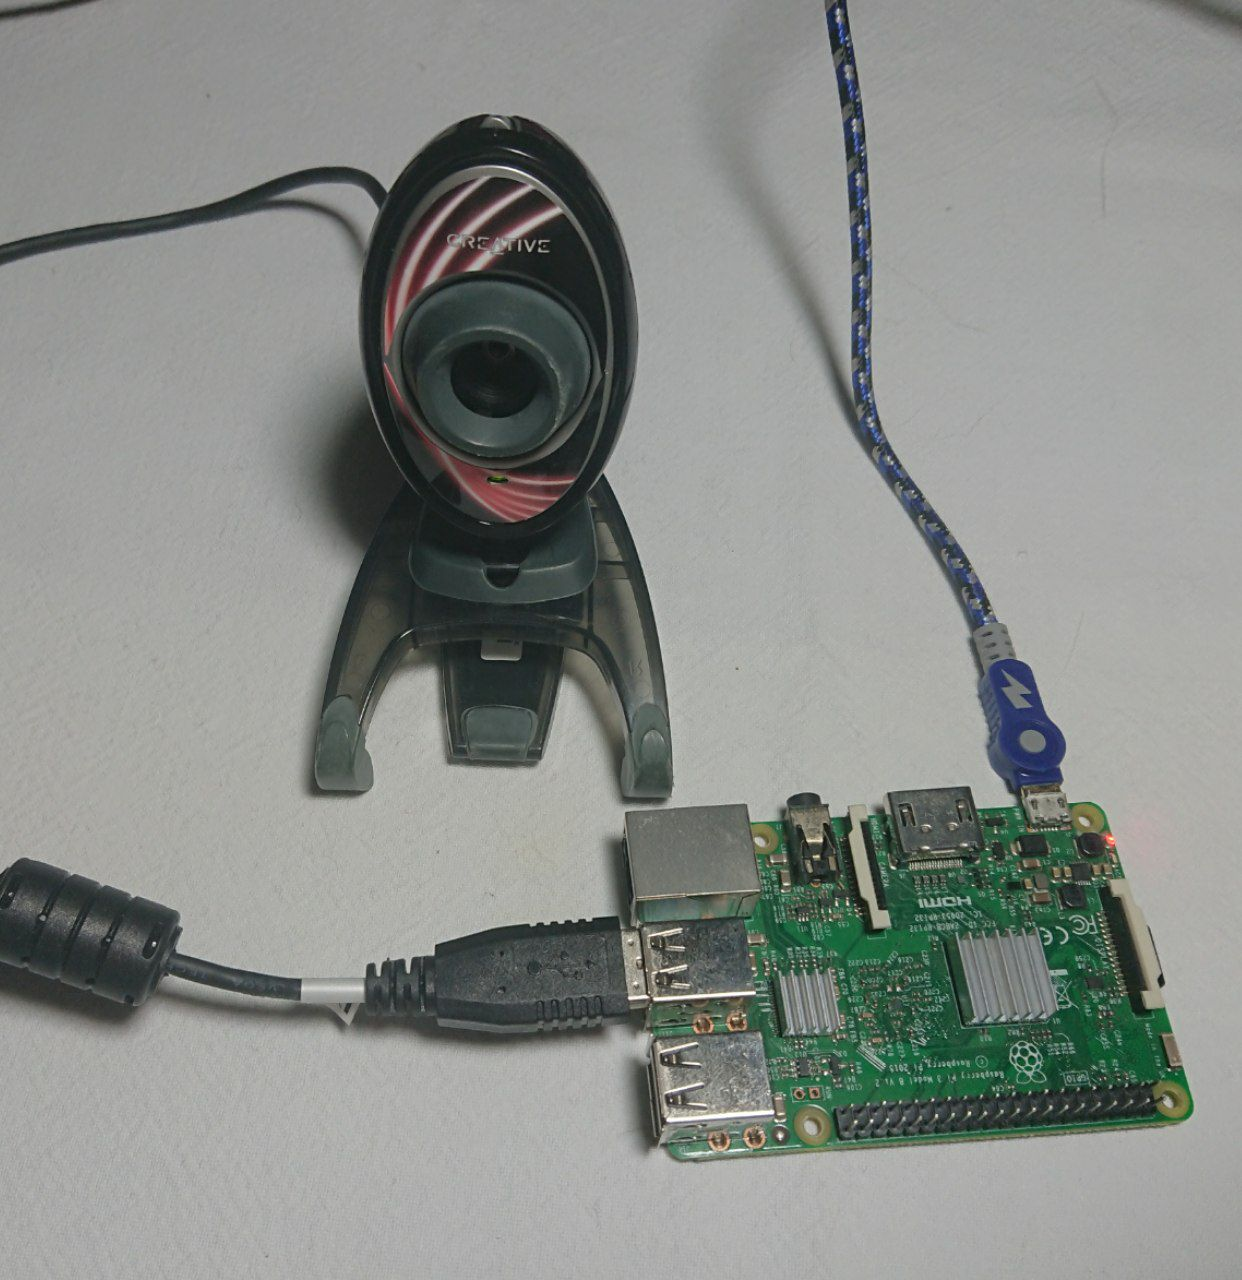
\includegraphics[width=1\textwidth]{Images/SmartCam.jpeg}
        \end{figure}
        
        %CORS LATO CONSOLE
        \begin{figure}[H]
            \caption{Prototipo Smart Collar}
            \label{fig:SmartCollar}
            \centering
            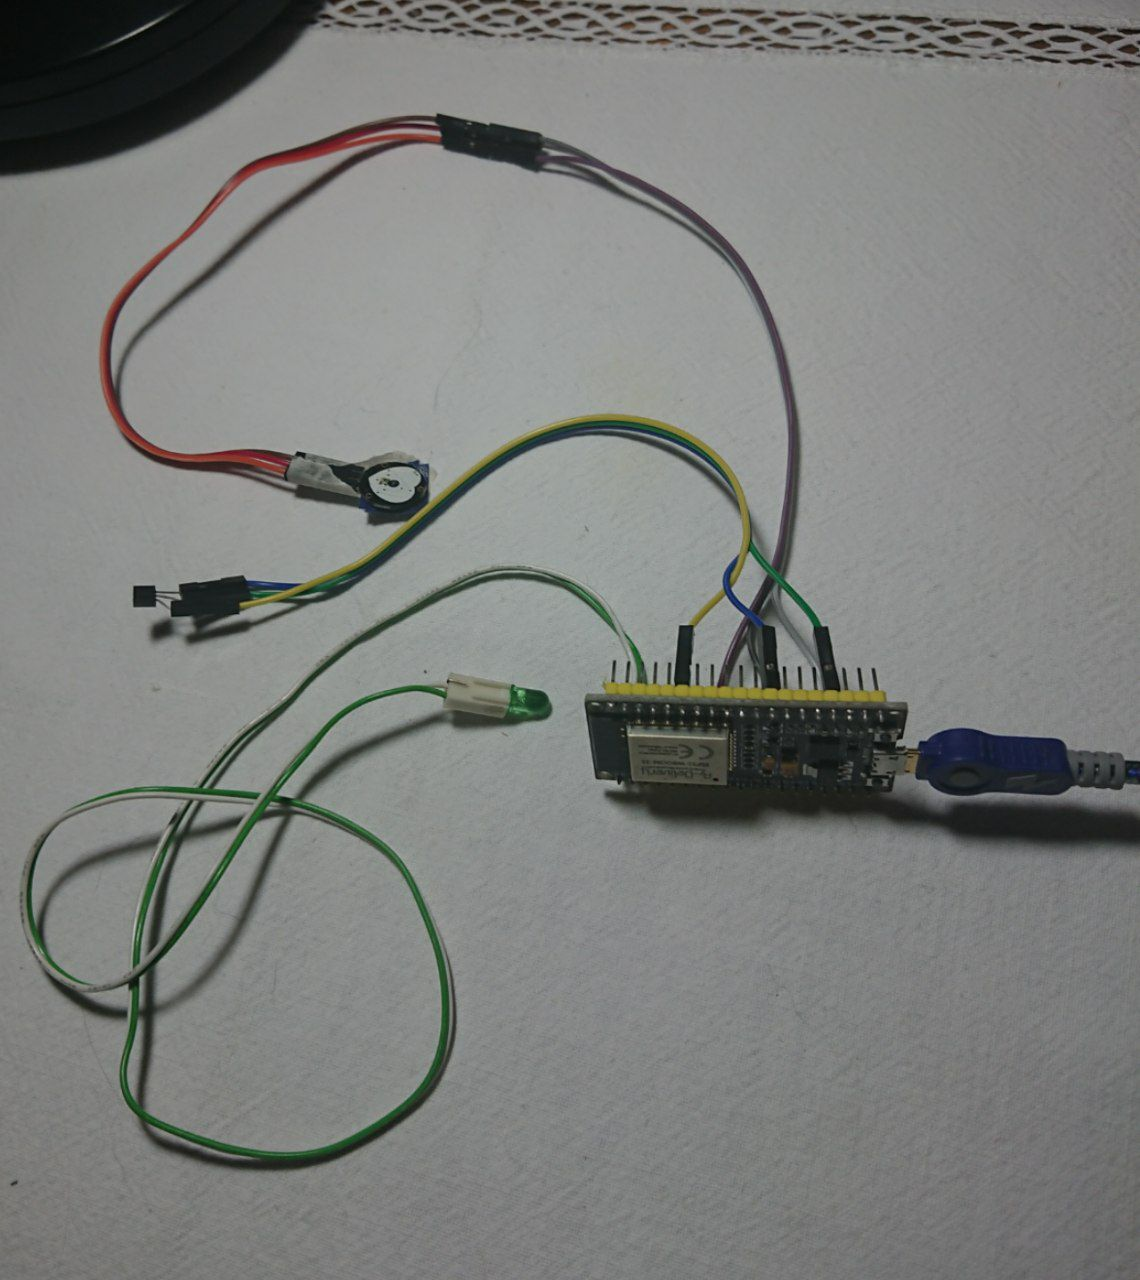
\includegraphics[width=1\textwidth]{Images/SmartCollar.jpeg}
        \end{figure}
        
        %CORS LATO CONSOLE
        \begin{figure}[H]
            \caption{Prototipo Smart Cage}
            \label{fig:SmartCage}
            \centering
            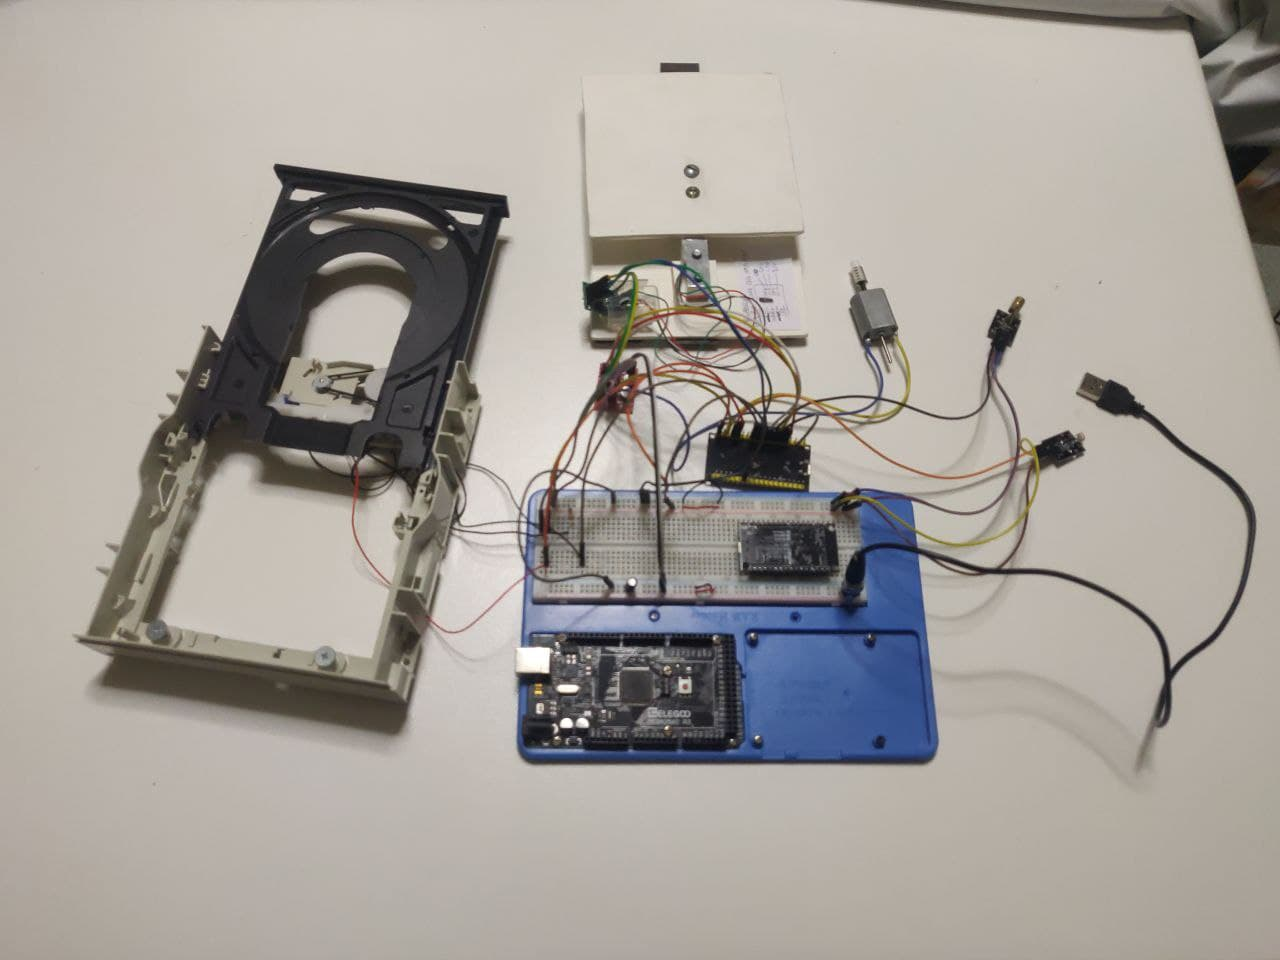
\includegraphics[width=1\textwidth]{Images/SmartCage.png}
        \end{figure}